%\documentclass[draft]{beamer}
\documentclass{beamer}
  
\usepackage{thumbpdf}           % Thumbnails for PDF versions
\usepackage{hyperref}
\usepackage{pgf}
\usepackage{tikz}
\usepackage{bm}
\usepackage{movie15}
\usepackage{textcomp}

\definecolor{green::dark}{rgb}{0.,0.7,0}

\title{Advanced Amateur Radio Licence: Part IV}
\subtitle{Antenna Matching}
\author{Rupert Brooks}

%%%%%%%%%%%%%%%%%%%%%%%%%%%%%%%%%%%%%%%%%%%%%%%%%%%%%%%%%%%%%%%%%%%%%%%%%%%%%%%%%%
%\setbeamertemplate{navigation symbols}{}
%\setbeamertemplate{frametitle}[default][right]
\setbeamertemplate{frametitle}{
\begin{flushright}
\insertframetitle\\
{\small \insertframesubtitle}
\end{flushright}
}

\setbeamertemplate{footline}[frame number]

\usefonttheme{professionalfonts}

%\setbeamertemplate{background}
%{
%\put(-10,0){
%\includegraphics[height=0.2\paperwidth]{logo.jpg}
%}%
%\put(0,2){
%\includegraphics[width=0.5in]{MICCAI_Logo_CMYK.pdf}
%}


%%%%%%%%%%%%%%%%%%%%%%%%%%%%%%%%%%%%%%%%%%%%%%%%%%%%%%%%%%%%%%%%%%%%%%%%%%%%%%%%%%
\def\lemma{{\large  \usebeamercolor[fg]{titlelike} Lemma\\}}
\def\proof{{\large  \usebeamercolor[fg]{titlelike}  Proof\\}}
\def\endproof{\qed}

\def\point#1{{\large  \usebeamercolor[fg]{titlelike}  #1\\}}
\def\herepoint#1{{\large  \usebeamercolor[fg]{titlelike}  #1}}

\def\emph#1{{\usebeamercolor[fg]{titlelike}  #1}}

%%%%%%%%%%%%%%%%%%%%%%%%%%%%%%%%%%%%%%%%%%%%%%%%%%%%%%%%%%%%%%%%%%%%%%%%%%%%%%%%%%
\begin{document}

%%%%%%%%%%%%%%%%%%%%%%%%%%%%%%%%%%%%%%%%%%%%%%%%%%%%%%%%%%%%%%%%%%%%%%%%%%%%%%%%%%
\begin{frame}
\maketitle
\end{frame}


%%%%%%%%%%%%%%%%%%%%%%%%%%%%%%%%%%%%%%%%%%%%%%%%%%%%%%%%%%%%%%%%%%%%%%%%%%%%%%%%%%
%% \section*{Outline}
%% \begin{frame}[allowframebreaks]
%% \frametitle{Outline}
%% \tableofcontents
%% \end{frame}
%%%%%%%%%%%%%%%%%%%%%%%%%%%%%%%%%%%%%%%%%%%%%%%%%%%%%%%%%%%%%%%%%%%%%%%%%%%%%%%%%%

\section*{Outline}

\begin{frame}{Outline}{}
\tableofcontents
\end{frame}
%%%%%%%%%%%%%%%%%%%%%%%%%%%%%%%%%%%%%%%%%%%%%%%%%%%%%%%%%%%%%%%%%%%%%%%%%%%%%%%%%%
\section{Overview}

\begin{frame}{General}{}
Thinking about it from a transmission point of view
\begin{itemize}
\item Generate the RF signal: RF amp (covered last time)
\item Send it to an antenna: transmission line.  You might need an antenna tuner and or and impedance matching antenna feed too.
\item Radiate it: Antennas, radiation, etc
\end{itemize}
... obviously reception is the reverse.
\end{frame}

\begin{frame}{Safety}{}
\begin{itemize}
\item Remember commandment VII of the ten commandments of electrical safety

\begin{quote}
Work thou not on energized equipment without proper procedures, for
if thou dost so, thy shipmates will surely be buying beers for thy widow
and consoling her in ways not generally acceptable to thee.
\end{quote}
\small{\url{http://goatlocker.org/resources/nav/safety.htm}}

\item The business end of an RF amp is a hazardous place to be when it is on.
\item Installations should be physically secured, to protect the curious.
\item Transmitter should be off (and maybe lockout) when working on waveguides, feed horns, etc.
\end{itemize}
\end{frame}


\section{Getting to the antenna}

\begin{frame}{Antenna tuner}{}
\begin{itemize}
\item Generally suitable for 50 ohm input
\item L type: for high output impedance.  Small matching range
\item $\Pi$ type: matches low to high impedance.  One inductor and two caps or vice versa.  Wide matching range.
\item $\Pi$-L type: like $\Pi$ but with greater harmonic suppression.
\item Series / transformer types.  Matches low to high impedances.
\end{itemize}
\end{frame}

\begin{frame}{Transmission Line / Waveguide}{}
\begin{itemize}
\item RF moves slower (typical, 2/3 speed) along transmission line than air.  Velocity factor is speed of signal in line / speed of light in vacuum.  Dielectric is the determining factor.
\item a {quarter-wave stub} shows impedance the opposite of what it actually is.  (Shorted - high impedance, open - low impedance)
\item a {half-wave stub} shows impedance the same as what it really is. (Shorted - low impedance, open - high impedance)
\item a {\em waveguide} is like a pipe for RF.  Works best at high frequencies, acts as a high pass filter.  
\item {\em stripline} Conductor sandwiched between two dielectrics.  Like a flattened coax.
\item {\em microstripline} printed circuit transmission line.  Generally a conducting strip separated from a ground plane on the other side of the board. Relatively poorly shielded.
\item Lots of useful info at http://www.microwaves101.com/encyclopedia/transmission.cfm

\end{itemize}
\end{frame}

\begin{frame}{Antenna feed}{}
\begin{itemize}
\item Gamma match: unbalanced feed - coax braid to the center, and center conductor along one side via a capacitor with an adjustable parallel rod. 
\item T match: like two gamma matches, one on each side.
\item Stub match: a short section of line open or shorted connected across the feed line at a specific distance from the antenna feed point.
\end{itemize}
\end{frame}

\section{Antennas}

\begin{frame}{The Half wave Dipole}{}
\begin{itemize}
\item Normally fed in the middle
\item The current is highest in the center and lowest at the ends
\item The voltage is highest at the end and lowest in the middle.
\item The impedance is highest at the end and lowest in the middle.
\item When calculating the physical length, it is {\em shorter} than the wavelength in free space.  Use 95\% on the test.
\end{itemize}
\end{frame}

\begin{frame}{The Half wave Dipole}{cont.}
\begin{centering}
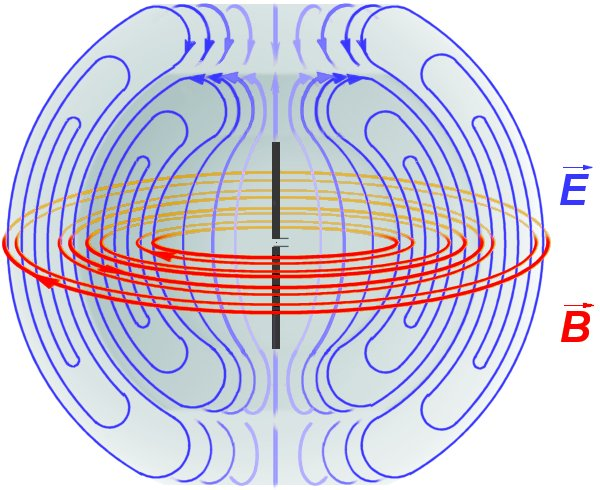
\includegraphics[width=0.4\textwidth]{images/dipolefield.jpg}

\small{\url{https://en.wikipedia.org/wiki/File:Felder_um_Dipol.jpg}}
\end{centering}
\begin{itemize}
\item Theoretical gain 2.1 dBi
\item If it is horizontal less than a half wavelength above ground, ground reflection distorts the radiation pattern and there is little directivity
\item above 1 $\lambda$ above ground impedance 75$\Omega$
\end{itemize}
\end{frame}

\begin{frame}{The Yagi-Uda}{}
\begin{centering}
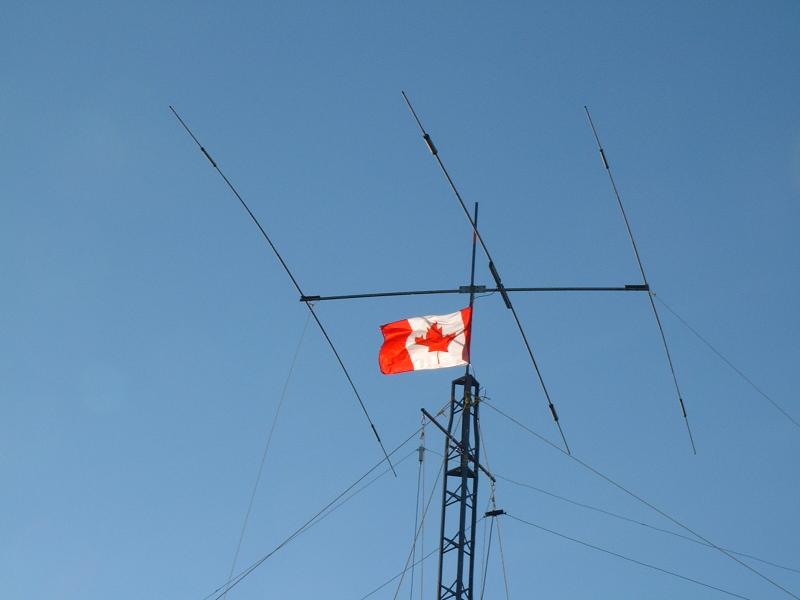
\includegraphics[width=0.4\textwidth]{images/yagi.jpg}

\small{\url{https://en.wikipedia.org/wiki/File:Montreal-tower-top.thumb2.jpg}}
\end{centering}
\begin{itemize}
\item Only one driven element, one reflector, and one or more directors
\item Takeoff angle decreases with increasing height - less than 30degrees preferred for long distance.
\end{itemize}
\end{frame}

\begin{frame}{Polarization}{}
\begin{itemize}
\item Electromagnetic waves have both a magnetic and electric field, at right angles.
\item Orientation of the electric field determines the polarization
\item Orientation of radiating elements determines orientation of electric field, and thus polarization
\item obvious types, horizontal, and vertical.  
\item line of sight communication will work best when polarization matches.
\item Circular polarization can be either left handed or right handed.  Crossed dipole and dual helical antennas can generate both.
\end{itemize}
\end{frame}

\begin{frame}{Radiated power}{}
\begin{itemize}
\item Effective radiated power (ERP)  
\begin{itemize}
\item is Transmitter output power less line loss plus antenna gain.
\item line loss and antenna gain in dB can be added and subtracted, then dB converted to a multiplier as 3dB is 2x
\end{itemize}
\item Radiation resistance 
\begin{itemize}
\item is the equivalent resistance that would dissipate the radiated power.
\item the Radiation resistance as a fraction of the total resistance is the antenna efficiency.
\item affected by antenna location, nearby objects and conductor length / diameter ratio

\end{itemize}

\end{itemize}
\end{frame}



%%%%%%%%%%%%%%%%%%%%%%%%%%%%%%%%%%%%%%%%%%%%%%%%%%%%%%%%%%%%%%%%%%%%%%%%%%%%%%%%%%

%\section{Modulation}

%\subsection{Rectifiers}
%\begin{frame}{Rectifiers}{}
%\end{frame}

%%%%%%%%%%%%%%%%%%%%%%%%%%%%%%%%%%%%%%%%%%%%%%%%%%%%%%%%%%%%%%%%%%%%%%%%%%%%%%%%%%
\end{document}
 
